\chapter{Compréhension et exploration des données}
\label{chap:eda}
\thispagestyle{plain}

\section{Objectifs de l'exploration}
Cette première étape vise à comprendre la structure du jeu de données, la distribution de la variable cible et les relations descriptives entre les variables candidates et la présence d'un AVC. L'exploration sert à formuler des hypothèses et à orienter les choix de préparation et d'évaluation ; elle ne permet, à elle seule, ni d'établir une causalité ni de valider un outil clinique.

\section{Présentation du jeu de données}
Le fichier brut contient \textbf{5\,110 observations et 12 colonnes}. La cible binaire \texttt{stroke} indique si un AVC est enregistré pour l'observation considérée (\texttt{stroke=1}) ou non (\texttt{stroke=0}). Les variables explicatives couvrent l'âge, l'hypertension, les antécédents de maladie cardiaque, le niveau moyen de glucose, l'indice de masse corporelle (IMC), ainsi que des caractéristiques démographiques et comportementales.

\begin{table}[H]
    \centering
    \caption{Nature des variables du jeu de données initial}
    \label{tab:eda-variable-types}
    \renewcommand{\arraystretch}{1.2}
    \begin{tabularx}{\textwidth}{@{}>{\raggedright\arraybackslash}p{3.1cm}X@{}}
        \toprule
        \textbf{Type} & \textbf{Variables}\\
        \midrule
        Identifiant & \texttt{id} (identifiant de ligne, non destiné à être utilisé comme prédicteur)\\
        Numérique & \texttt{age}, \texttt{avg\_glucose\_level}, \texttt{bmi}\\
        Binaire & \texttt{hypertension}, \texttt{heart\_disease}\\
        Catégoriel & \texttt{gender}, \texttt{ever\_married}, \texttt{work\_type}, \texttt{Residence\_type}, \texttt{smoking\_status}\\
        Cible & \texttt{stroke} (0 : aucun AVC enregistré ; 1 : AVC enregistré)\\
        \bottomrule
    \end{tabularx}
\end{table}

Le jeu brut ne comporte ni doublon de ligne ni doublon d'identifiant. La colonne \texttt{id} est donc utile pour l'identification des enregistrements, mais ne porte pas de caractéristique clinique pertinente et sera écartée des variables d'entrée. L'exploration relève également une modalité \texttt{Other} pour le genre, représentée par une seule observation ; son traitement est documenté dans l'étape de préparation afin d'éviter qu'une modalité quasi isolée ne perturbe l'encodage.

\section{Déséquilibre de la variable cible}
La distribution de \texttt{stroke}, représentée à la figure~\ref{fig:target_dist}, met en évidence une forte rareté des cas positifs.

\begin{table}[H]
    \centering
    \caption{Répartition de la cible dans le jeu brut}
    \label{tab:eda-target-distribution}
    \begin{tabular}{@{}lrr@{}}
        \toprule
        \textbf{Classe} & \textbf{Effectif} & \textbf{Proportion}\\
        \midrule
        \texttt{stroke=0} & 4\,861 & 95,13\,\%\\
        \texttt{stroke=1} & 249 & 4,87\,\%\\
        \bottomrule
    \end{tabular}
\end{table}

\begin{figure}[H]
    \centering
    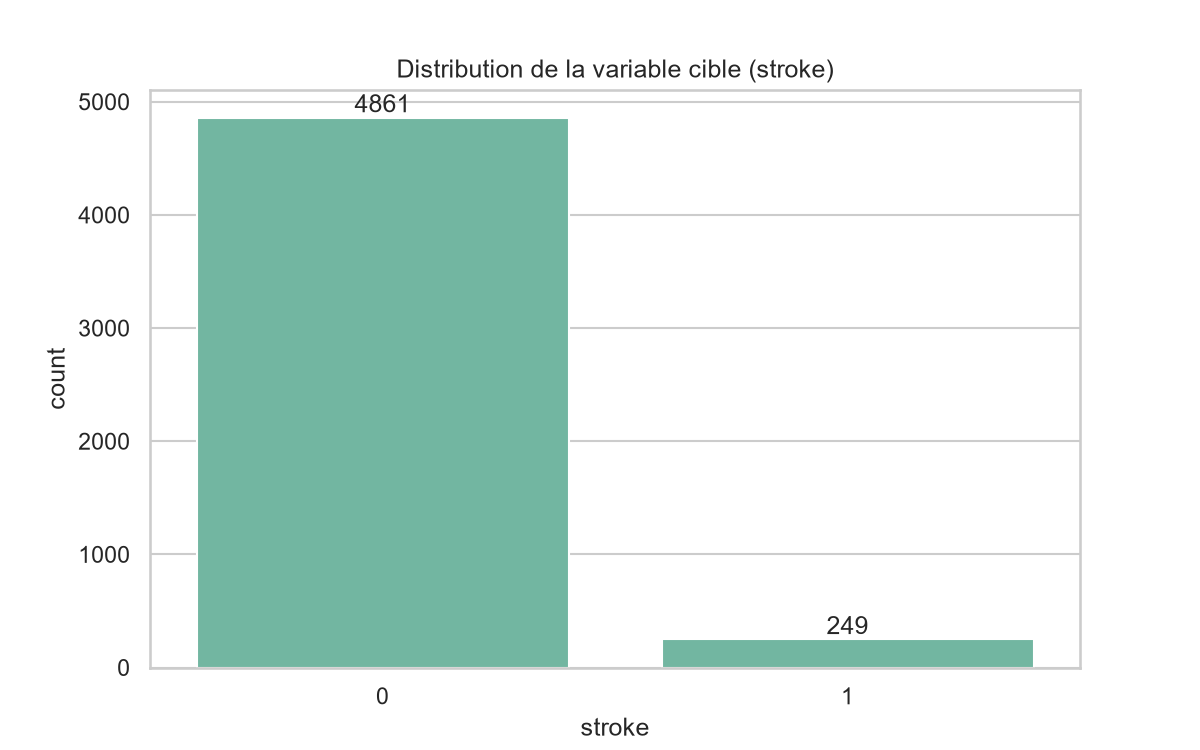
\includegraphics[width=0.72\textwidth]{02_target_distribution.png}
    \caption{Distribution de la variable cible \texttt{stroke}}
    \label{fig:target_dist}
\end{figure}

Cette asymétrie conditionne la suite du projet. Un modèle qui attribuerait la classe majoritaire à toutes les observations afficherait déjà environ 95\,\% d'exactitude, tout en manquant les 249 cas positifs. L'exactitude ne peut donc pas servir seule de critère de sélection. Le benchmark devra examiner spécifiquement le rappel de la classe AVC, la précision, la spécificité et des métriques adaptées aux classes déséquilibrées, notamment la PR-AUC. La stratégie de modélisation intégrera également une pondération des classes ou un rééchantillonnage réalisé uniquement dans les plis d'entraînement.

\section{Variables numériques et tests de Mann--Whitney}
\subsection{Forme des distributions}
Les distributions numériques présentées à la figure~\ref{fig:eda-numeric-distributions} montrent des formes différentes selon la variable. L'âge est relativement peu asymétrique (skewness de $-0{,}14$), tandis que le niveau moyen de glucose et l'IMC présentent une asymétrie à droite (respectivement $1{,}57$ et $1{,}06$). Une comparaison fondée exclusivement sur les moyennes ou sur une hypothèse de normalité serait donc insuffisante pour caractériser les écarts entre groupes.

\begin{figure}[H]
    \centering
    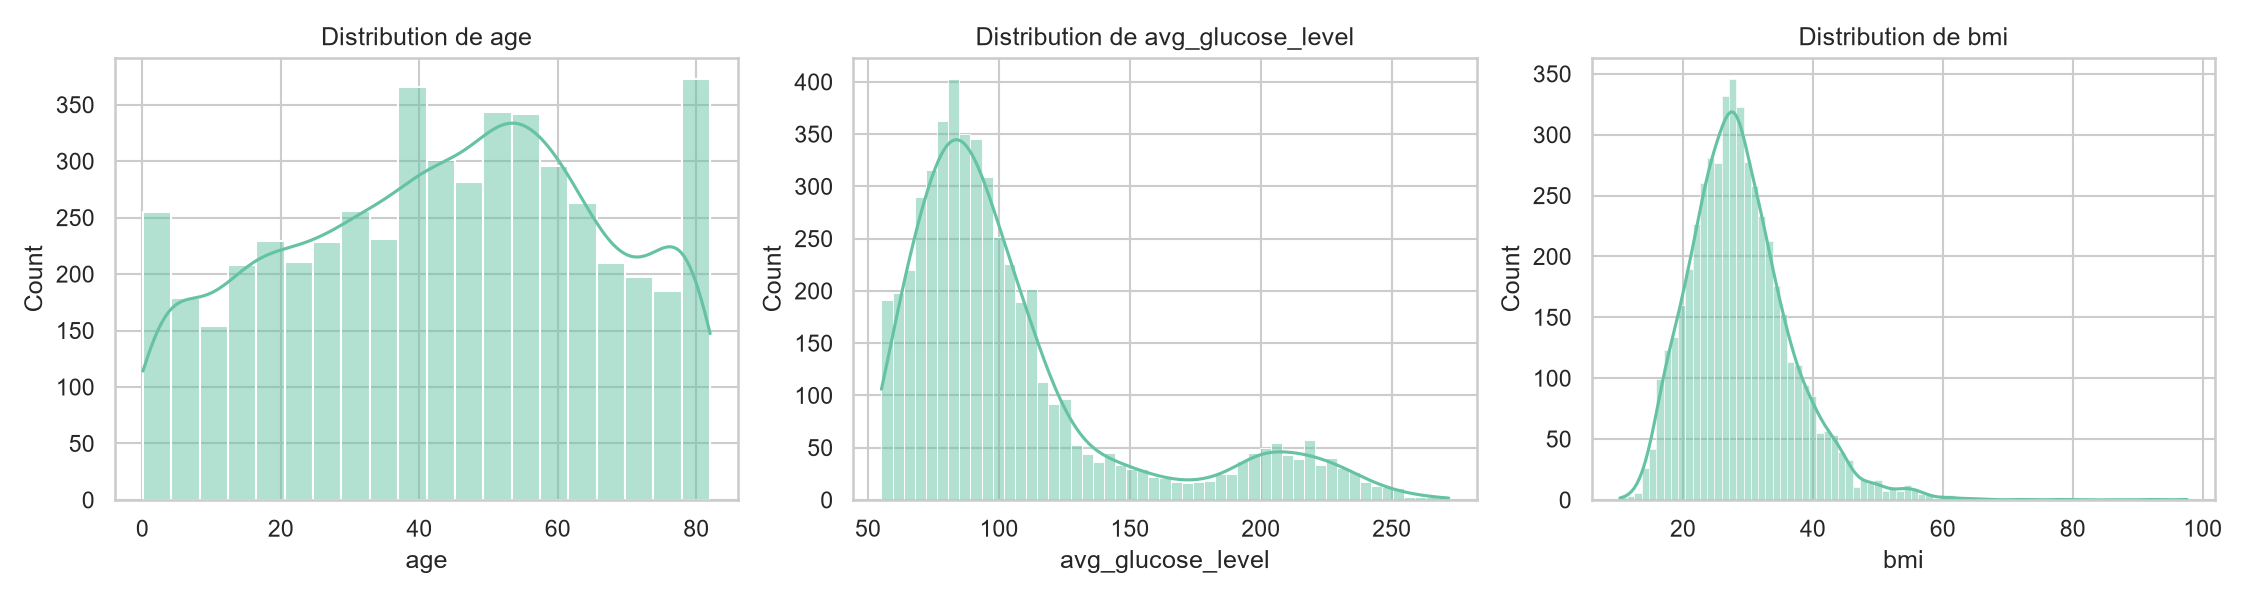
\includegraphics[width=0.92\textwidth]{03_num_distributions.png}
    \caption{Distributions des variables numériques dans le jeu brut}
    \label{fig:eda-numeric-distributions}
\end{figure}

\subsection{Comparaison exploratoire des groupes}
Pour comparer les observations des classes \texttt{stroke=0} et \texttt{stroke=1}, le notebook applique le test non paramétrique de Mann--Whitney à l'âge, au niveau moyen de glucose et à l'IMC. Ce test, fondé sur les rangs, permet de rechercher une différence de distribution sans imposer une loi normale aux mesures. Le tableau~\ref{tab:eda-mann-whitney} présente, à titre descriptif, les moyennes calculées pour chaque classe et les valeurs $p$ obtenues.

\begin{table}[H]
    \centering
    \caption{Comparaison des variables numériques selon la cible}
    \label{tab:eda-mann-whitney}
    \renewcommand{\arraystretch}{1.15}
    \begin{tabular}{@{}lrrr@{}}
        \toprule
        \textbf{Variable} & \textbf{Moyenne, classe 0} & \textbf{Moyenne, classe 1} & \textbf{Valeur $p$}\\
        \midrule
        \texttt{age} & 41,97 & 67,73 & $3{,}73 \times 10^{-71}$\\
        \texttt{avg\_glucose\_level} & 104,80 & 132,54 & $3{,}64 \times 10^{-9}$\\
        \texttt{bmi} & 28,82 & 30,47 & $1{,}03 \times 10^{-4}$\\
        \bottomrule
    \end{tabular}
\end{table}

Les trois valeurs $p$ sont très inférieures au seuil exploratoire de 0,05 : les distributions observées diffèrent donc entre les groupes dans cet échantillon. L'âge présente l'écart de moyenne le plus marqué, suivi du niveau moyen de glucose ; l'écart de moyenne d'IMC est plus limité, mais le test détecte également une différence de rangs. Ces résultats ne démontrent ni un lien causal ni une capacité de prédiction indépendante : ils ne tiennent pas compte des interactions entre variables et doivent être interprétés en tenant compte du déséquilibre de la cible et des données manquantes. Les courbes de densité de la figure~\ref{fig:eda-numeric-by-stroke} complètent cette comparaison visuelle.

\begin{figure}[H]
    \centering
    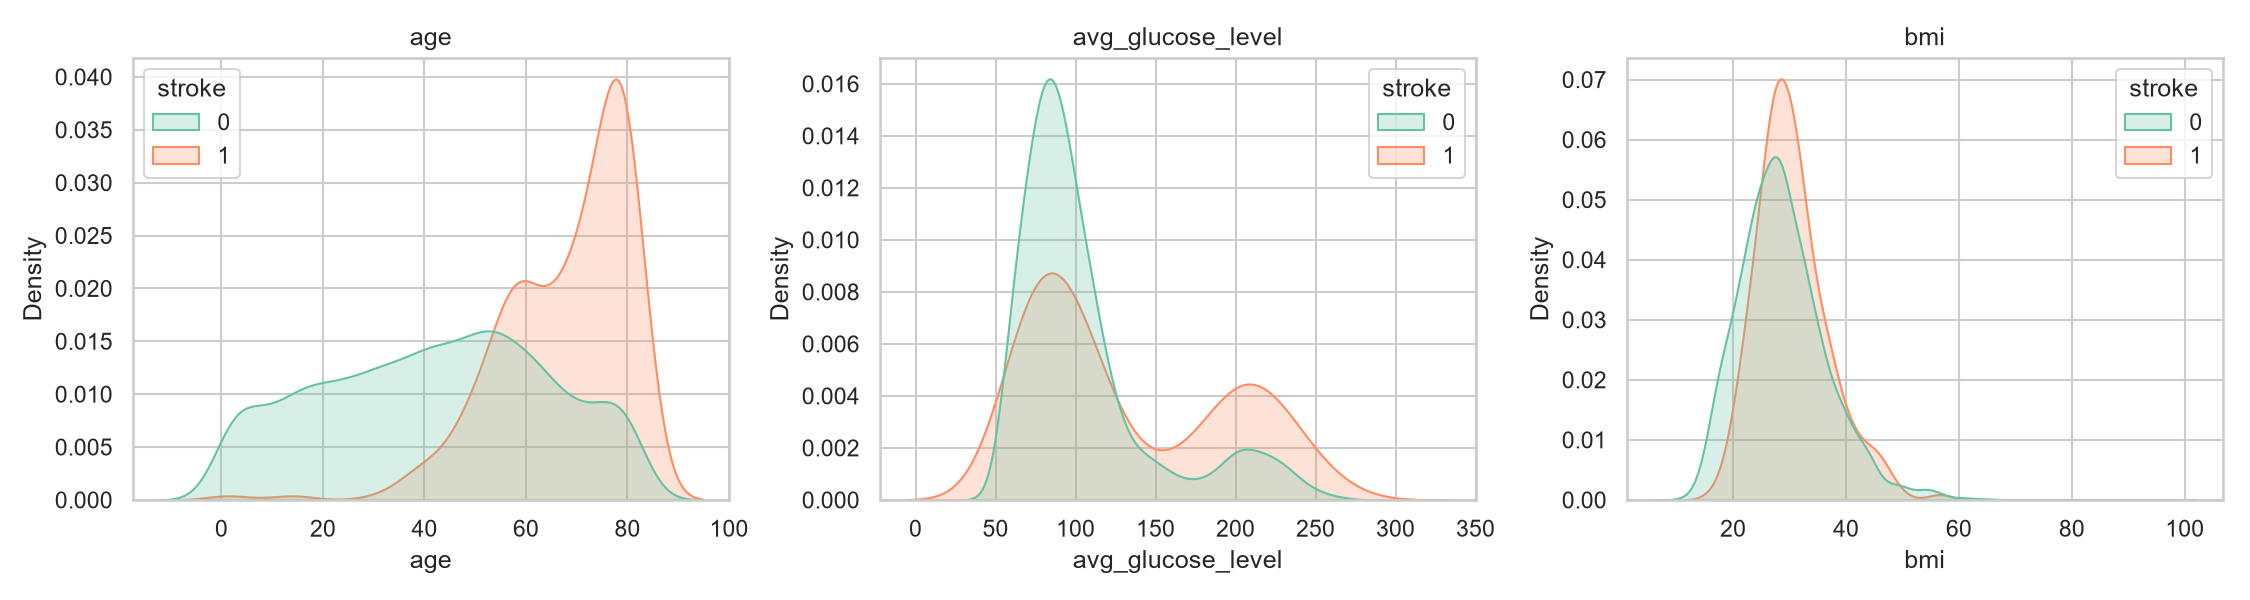
\includegraphics[width=0.92\textwidth]{05_num_kde_by_stroke.png}
    \caption{Distributions des variables numériques par classe de \texttt{stroke}}
    \label{fig:eda-numeric-by-stroke}
\end{figure}

\section{Valeurs manquantes de l'IMC : un signal à préserver}
La seule variable présentant des valeurs manquantes dans l'exploration est l'IMC : \textbf{201 valeurs, soit 3,93\,\%} des observations. Leur répartition selon la cible est particulièrement informative :

\begin{table}[H]
    \centering
    \caption{Prévalence observée de la classe AVC selon la disponibilité de l'IMC}
    \label{tab:eda-bmi-missing}
    \renewcommand{\arraystretch}{1.15}
    \begin{tabular}{@{}lrrr@{}}
        \toprule
        \textbf{Disponibilité de l'IMC} & \textbf{Effectif} & \textbf{Part du jeu} & \textbf{Taux de \texttt{stroke=1}}\\
        \midrule
        IMC renseigné & 4\,909 & 96,07\,\% & 4,26\,\%\\
        IMC manquant & 201 & 3,93\,\% & \textbf{19,90\,\%}\\
        \bottomrule
    \end{tabular}
\end{table}

Le taux d'AVC parmi les observations sans IMC est donc supérieur de 15,64 points de pourcentage au taux observé lorsque l'IMC est renseigné. Dans le cadre de ce jeu, ce contraste contredit la plausibilité d'une hypothèse stricte de données manquantes complètement au hasard (MCAR), selon laquelle l'absence de mesure serait indépendante des variables observées et non observées \cite{rubin1976missing}. Il s'agit d'un constat descriptif : il ne permet pas, à lui seul, d'identifier le mécanisme de non-réponse ni de distinguer un mécanisme MAR d'un mécanisme MNAR. Une analyse causale de la raison de l'absence de mesure demanderait des informations supplémentaires sur le processus de collecte.

Imputer directement les valeurs manquantes par une médiane ferait disparaître le fait qu'une mesure était absente. Pour éviter cette perte d'information, la préparation crée donc une variable indicatrice binaire \texttt{bmi\_missing} avant l'imputation : elle vaut 1 lorsque l'IMC initial est manquant et 0 autrement. L'IMC lui-même est ensuite imputé par la médiane estimée sur le jeu d'entraînement seulement (28,10 dans l'exécution documentée). Cette stratégie conserve un signal potentiellement utile sans prétendre que l'absence d'IMC cause l'AVC ; son apport devra être évalué hors échantillon et contrôlé contre le risque d'apprendre un biais propre au processus de collecte.

\section{Variables catégorielles, âge et valeurs atypiques}
\subsection{Associations observées pour les variables catégorielles}
Le notebook utilise des tests du $\chi^2$ sur les tableaux de contingence entre la cible et les variables catégorielles ou binaires. Les associations les plus marquées dans l'échantillon concernent les antécédents de maladie cardiaque ($p=2{,}09 \times 10^{-21}$), l'hypertension ($p=1{,}66 \times 10^{-19}$), le statut marital ($p=1{,}64 \times 10^{-14}$), le type d'emploi ($p=5{,}40 \times 10^{-10}$) et le statut tabagique ($p=2{,}09 \times 10^{-6}$). En revanche, les tests ne mettent pas en évidence d'association statistiquement significative pour le type de résidence ($p=0{,}298$) ni pour le genre ($p=0{,}790$). Ces tests restent exploratoires et ne prouvent pas de relation causale ; la modalité de genre représentée par une seule ligne invite en particulier à interpréter le résultat correspondant avec prudence.

\subsection{Gradient descriptif selon l'âge}
Le taux d'AVC observé augmente avec les tranches d'âge : il est de 0,22\,\% avant 18 ans, 0,45\,\% entre 18 et 40 ans, 4,10\,\% entre 40 et 60 ans, 12,96\,\% entre 60 et 80 ans et 19,83\,\% au-delà de 80 ans. Cette évolution descriptive concorde avec l'écart observé lors du test de Mann--Whitney, sans isoler l'effet propre de l'âge des autres facteurs associés.

\begin{figure}[H]
    \centering
    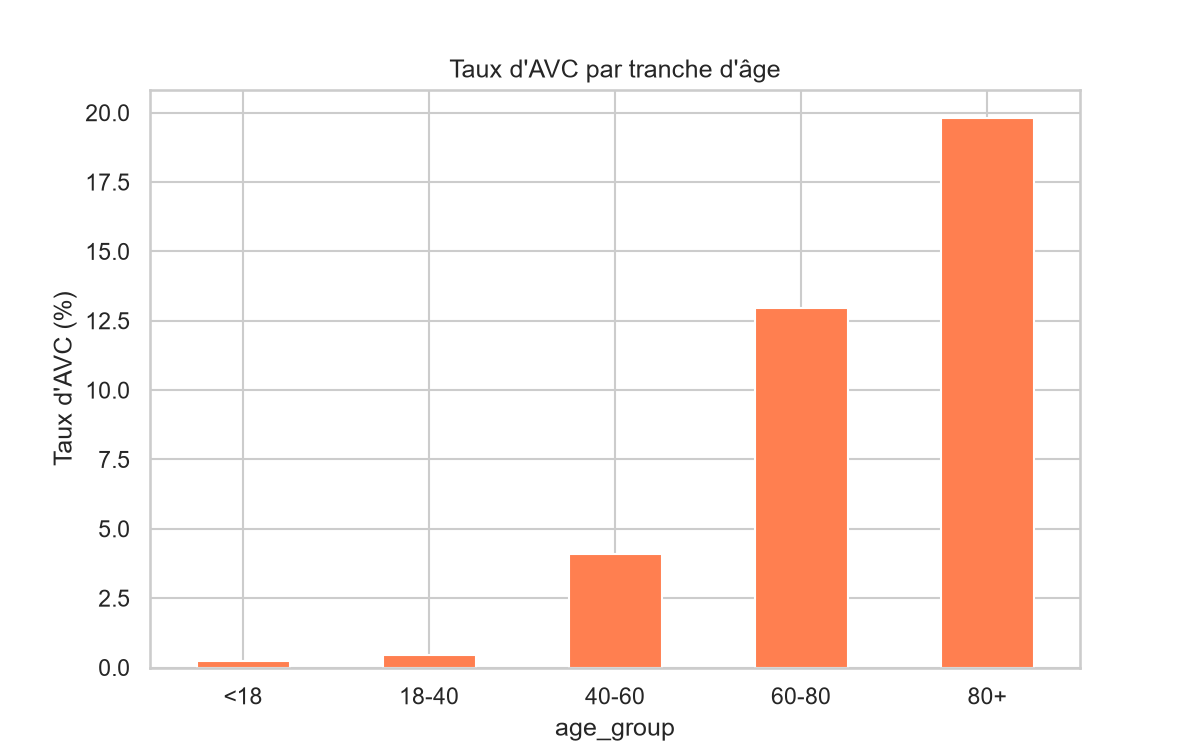
\includegraphics[width=0.78\textwidth]{06_stroke_rate_by_age.png}
    \caption{Taux d'AVC observé par tranche d'âge}
    \label{fig:eda-stroke-by-age}
\end{figure}

\subsection{Valeurs extrêmes et statut tabagique « Unknown »}
La règle de l'écart interquartile signale 627 valeurs extrêmes de glycémie moyenne (12,3\,\%) et 110 valeurs d'IMC (2,2\,\%). L'IMC maximal atteint 97,6, alors que la borne supérieure calculée par la règle IQR est de 47,5. Ces constats motivent un contrôle de l'influence des valeurs extrêmes ; le prétraitement retient un plafonnement de l'IMC à 60 plutôt qu'une suppression massive des lignes, afin de limiter l'effet des extrêmes tout en conservant les observations.

La modalité \texttt{Unknown} du statut tabagique concerne 1\,544 observations et est fortement représentée chez les jeunes (âge médian de 23 ans). Dans le prétraitement, 614 observations ayant un âge inférieur à 15 ans et un statut \texttt{Unknown} sont recodées en \texttt{never smoked}. Cette règle vise à éviter que l'absence de renseignement, attendue dans cette tranche d'âge, soit apprise comme une catégorie clinique équivalente chez les enfants. Elle constitue néanmoins une hypothèse de préparation, et non une observation vérifiée du comportement tabagique ; son effet doit être interprété avec prudence.

\section{Synthèse et implications pour la suite}
L'EDA met en évidence trois contraintes structurantes : la faible prévalence de la classe AVC, les différences de distributions entre les classes et l'association marquée entre l'absence d'IMC et la cible. Ces constats motivent l'emploi de métriques sensibles à la classe positive, la conservation de l'indicateur \texttt{bmi\_missing} et une préparation qui distingue les transformations déterminées a priori de celles apprises sur le train. Le chapitre suivant détaille le split des données, l'imputation et la standardisation, ainsi que les règles de nettoyage retenues.
